\begin{figure}[t]
\centering
\ifbilingual
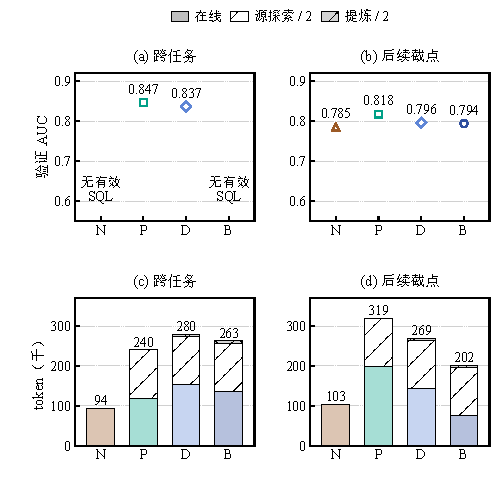
\includegraphics[width=\linewidth]{figures/memory-access-pilot-zh}
\else
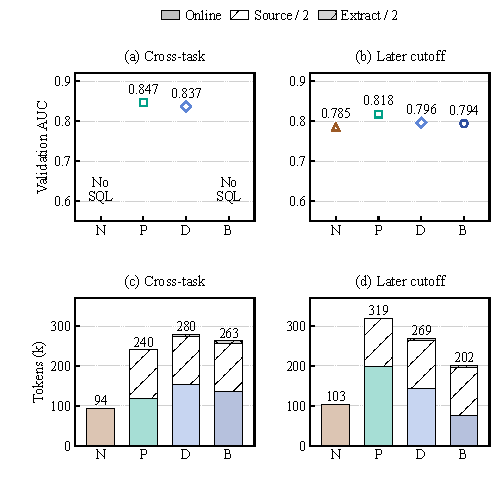
\includegraphics[width=\linewidth]{figures/memory-access-pilot}
\fi
\caption{\bt{Memory-access pilot: no memory (N), program only (P), definitions only (D), and both (B). Each arm runs once on user-engagement at the source cutoff and user-badge at the next cutoff. Missing solutions have no AUC point. Cost stacks charge source exploration over two targets and extraction to D/B only. Interrupted calls remain separately in the study ledger.}{记忆访问预实验：无记忆（N）、仅程序（P）、仅定义（D）及两者（B）。每组在源截点的user-engagement和下一截点的user-badge各运行一次。无有效方案不绘制AUC点。代价按两个目标摊销源探索，提炼仅计入D/B；中断调用的消耗在实验账本中单列保留。}}
\label{fig:memory-access-pilot}
\Description{Four panels show validation AUC and stacked token cost for two target settings. Cross-task N and B produce no valid SQL; their costs are retained. Lower panels include target-session tokens, one half of source exploration for P/D/B, and one half of extraction for D/B. This is one development run per cell, with no test-label scoring or confidence intervals.}
\end{figure}
